\section{\lr{Important Cameras}}

\subsection{توضیحات کلی}
در این قسمت، سعی کردم از الگوریتم 
HITS
استفاده‌ی بهتری کنم. این بار، راس‌های من تنها شامل دوربین‌ها می‌شوند. کافی است برای هر ماشین 
در هر روز، دوربین‌هایی که پشت هم می‌آیند را یک یال گراف در نظر بگیرم. دقت کنید 
که این یال‌ها جهت دارند. حال اگر از الگوریتم
HITS
استفاده کنیم،‌ می‌توانیم مهم‌ترین مکان‌هایی را پیدا کنیم، که به مکان‌های مهم دیگری مسیر دارند (
    بهترین 
    hub
    ها و 
    authority
    ها
). 

برای انجام دادن این کار، از تابع
lead
در 
sql
استفاده می‌کنیم. برای هر ردیف دوربین‌ ردیف بعدی را به 
df
اضافه می‌کنیم. این کار باید به ازای هر ماشین و هر روز جداگانه انجام شود. 
همچنین باید دقت کنید که داده باید قبل از این قسمت روی زمان مرتب شود (
    lead
    یک سینتکس 
    sql
    است. در صورتی که این قسمت گنگ است، کافی است توضیحات 
    lead
    را بخوانید
). 
نتیجه به صورت زیر شد: 

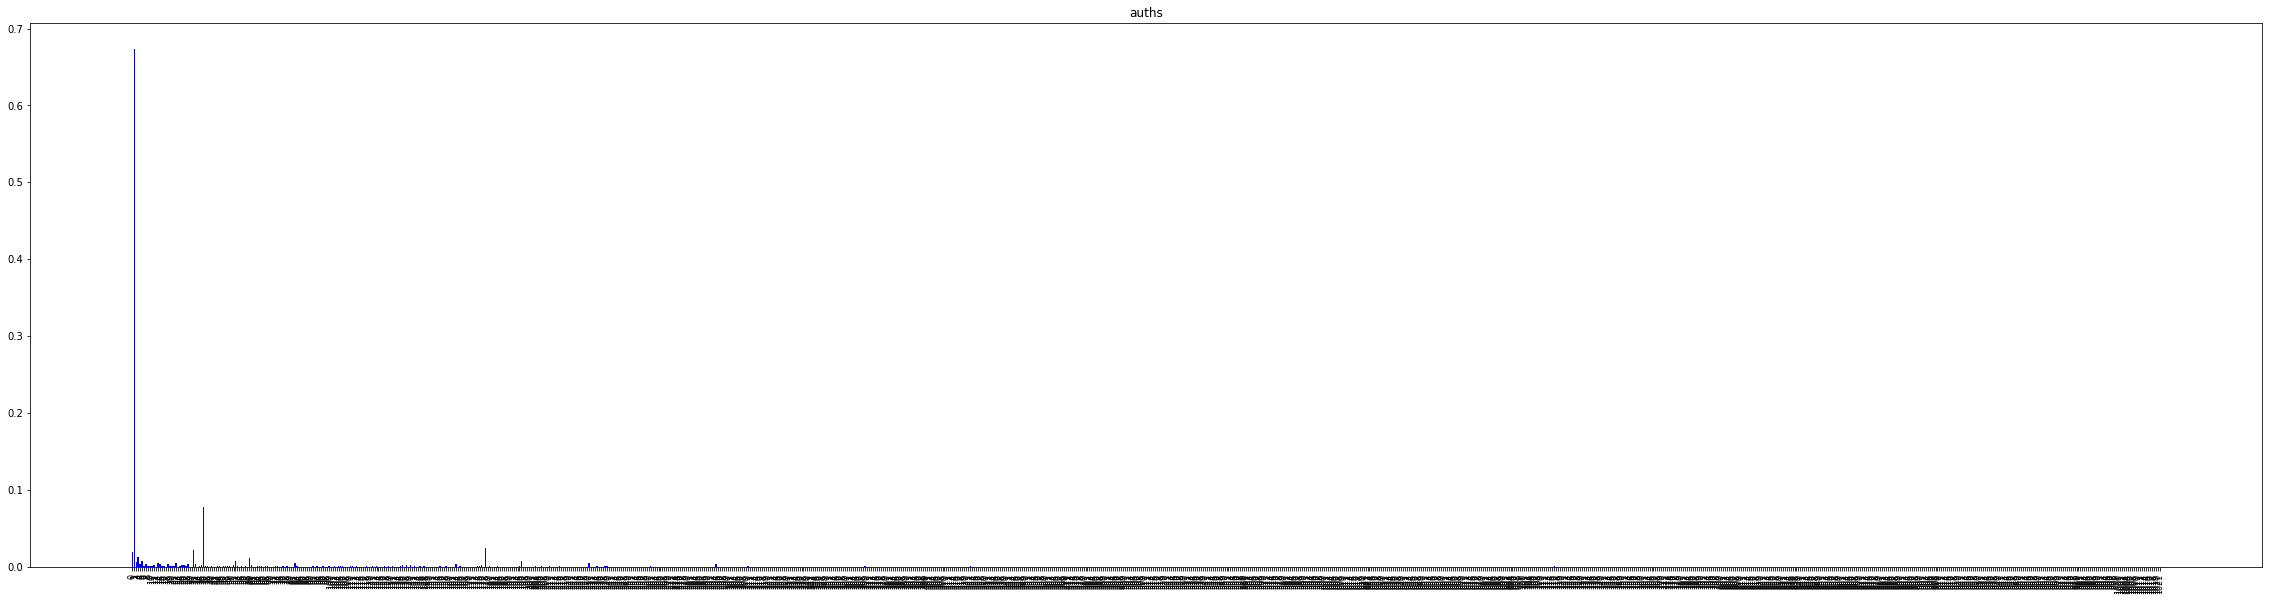
\includegraphics[scale = 0.2]{images/ImportantCameras/1.png}

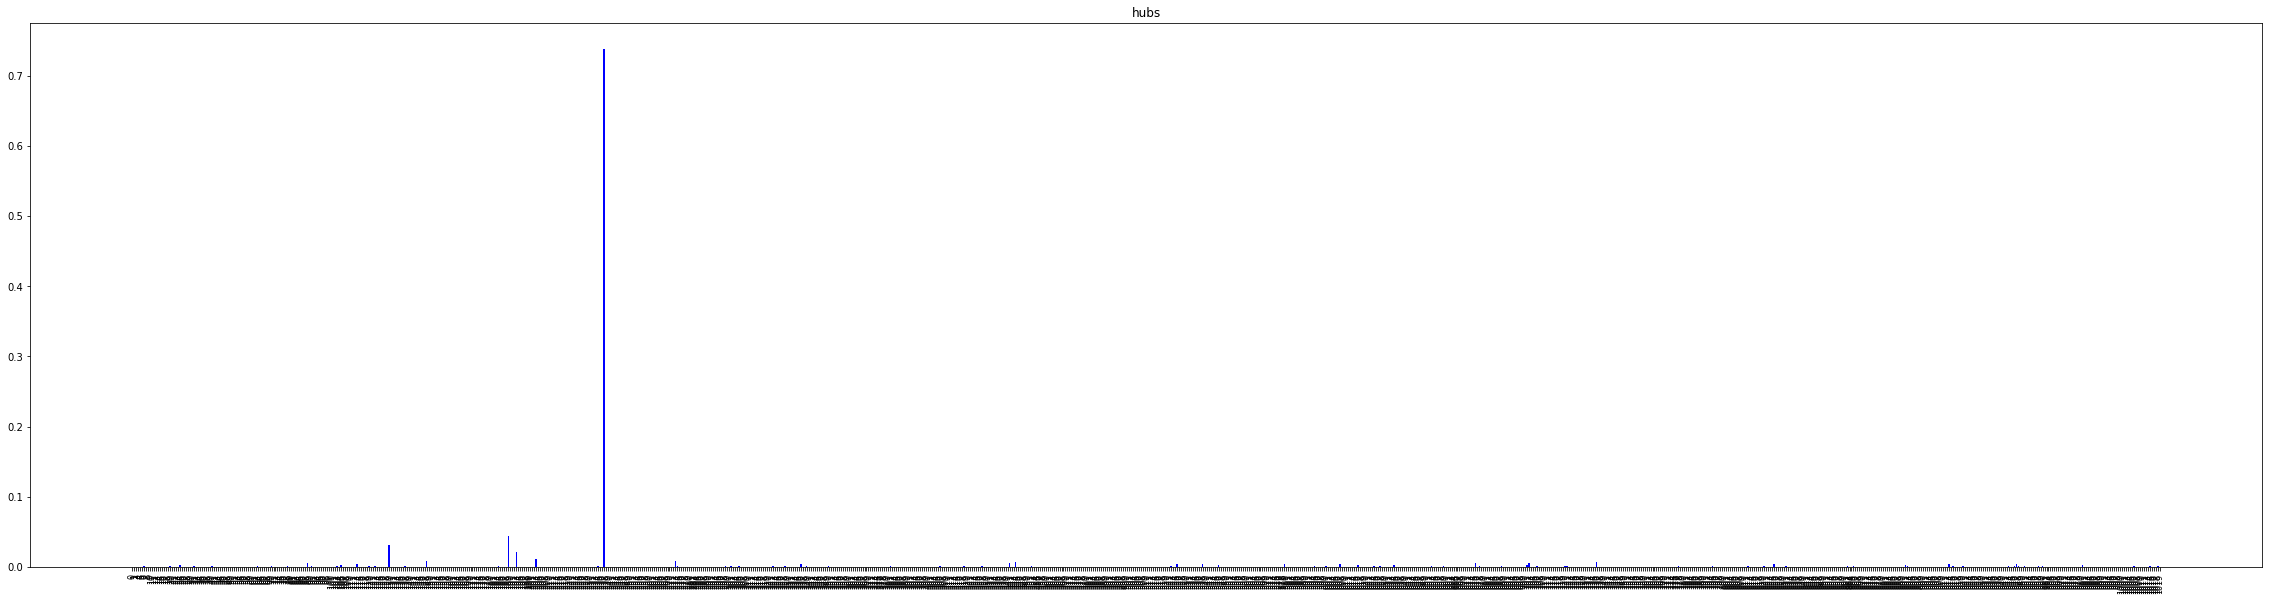
\includegraphics[scale = 0.2]{images/ImportantCameras/2.png}


\subsection{تحلیل نتایج}

همانطوری که می‌بینید، دو دوربین با اختلاف بهترین
hub
و
authority
شدند. لیست این دوربین‌ها به ترتیب در فایل 
jupyter
آمده است (البته دقت کنید که دوربین‌ها اندیس گذاری شده‌اند و اندیس‌ آن‌ها را برنگرداندم). 
نکته‌ی جالبی که وجود دارد این است که با این که دوربین‌ها به ترتیب کل تکرار شدن 
شماره گذاری شده‌اند، اما بهترین 
authority
۴۰ 
مین دوربین پرتکرار ما بوده است (یعنی با این که ۳۹ دوربین از آن پر تکرار تر بوده‌اند، اما بهترین 
authority 
شده است). 
